% This template has been taken and adapted from ICML 2021 submission file available under Creative Commons CC BY 4.0.

\documentclass{article}

\input{source/preamble}
\usepackage[accepted]{source/icml2021}

\setlength{\textfloatsep}{6pt plus 1pt minus 2pt}
\setlength{\floatsep}{6pt plus 1pt minus 2pt}
\setlength{\intextsep}{6pt plus 1pt minus 2pt}
\setlength{\abovecaptionskip}{3pt}
\setlength{\belowcaptionskip}{-2pt}

\newcommand{\sta}{\textsc{STA}}
\newcommand{\bartft}{BART-FT}
\newcommand{\best}[1]{{\bfseries\boldmath #1}}

\icmltitlerunning{EE-559 Deep Learning: Group Mini-Project, Group 31}

\begin{document}

\twocolumn[
\icmltitle{From Censorship to Detoxification: Rewriting Harmful Memes}

\begin{icmlauthorlist}
\icmlauthor{Alex Dell'Orto}{ch} \quad
\icmlauthor{Christian Garzone}{ch} \quad
\icmlauthor{Dario Liuzzo}{ch}
\end{icmlauthorlist}

\icmlaffiliation{ch}{EPFL}
\vskip 0.05in
\centering
Group 31, EE-559: Deep Learning, 2026
\vskip 0.18in
]

\printAffiliationsAndNotice{}

\begin{abstract}
Harmful memes are often toxic because image and text jointly imply an
identity-based attack. Instead of detecting and removing such content, we study
text detoxification: given a meme image and caption, produce a safer caption
that preserves the topic and image-text coherence. Our system uses LLaVA-NeXT
as a multimodal teacher to generate structured explanations and pseudo-rewrites,
then distills this behavior into a LoRA-adapted BART-large student. The main
deployment contribution is a CLIP Proxy + BART path that maps CLIP image/text
features to BART encoder soft tokens, avoiding a large VLM/LLM at inference.
On 280 held-out memes, the full BART student reaches $0.963\pm0.006$ Text
\sta{} and $0.207\pm0.006$ \sta{} delta across five seeds, compared with the
single reported DetoxLLM-7B baseline at 0.940 and 0.184. The proxy obtains the
highest BERTScore and CLIPScore ($0.581\pm0.020$, $0.638\pm0.002$), suggesting
stronger source retention and image alignment, but lower Text \sta{} shows
weaker toxicity control.\\
\textbf{Keywords:} meme detoxification, multimodal learning, text rewriting,
distillation, CLIP, BART.
\end{abstract}

\section{Introduction}
\label{sec:intro}

Hateful meme moderation is usually framed as classification: predict whether an
image-text pair is harmful and then remove or suppress it
\cite{kiela2020hateful,li2019visualbert}. This is necessary but incomplete.
Meme captions can be ambiguous alone, while the image supplies the target,
stereotype, or implied insult. A pure text detoxifier can miss that interaction;
a pure detector does not preserve a benign version of the communicative intent.

We formulate harmful meme moderation as \emph{text rewriting}. Given a meme
image and overlaid text, the goal is to rewrite the text so that the harmful
framing is reduced while the topic, short meme style, and visual compatibility
remain recognizable. This raises two questions. First, can multimodal teacher
explanations supervise a compact meme rewriter? Second, can CLIP-derived soft
encoder states provide a VLM-free inference path that keeps useful visual
grounding without running a large generator?

Our contributions are threefold. First, we implement an explain-then-rewrite
pipeline that uses LLaVA-NeXT \cite{liu2024llavanext} to produce target groups,
visual evidence, implicit meanings, and pseudo-detoxified captions. Second, we
fine-tune BART-large \cite{lewis2020bart} with LoRA \cite{hu2022lora} on these
meme-specific pseudo-labels and compare it to DetoxLLM-7B
\cite{khondaker2024detoxllm} and non-fine-tuned BART. Third, we introduce a
deployment-oriented CLIP Proxy + BART path: CLIP \cite{radford2021learning}
encodes the image and text, a small MLP predicts BART encoder-memory soft
tokens, and the fine-tuned BART decoder generates the rewrite without running
LLaVA or another 7B language model at inference.

\section{Related Work}
\label{sec:related}

\textbf{Hateful meme understanding.} The Hateful Memes benchmark showed that
multimodal reasoning is required because unimodal cues are deliberately
confounded \cite{kiela2020hateful}. VisualBERT \cite{li2019visualbert} and CLIP
\cite{radford2021learning} provide useful image-text representations, but the
standard objective is still detection. Our work differs by producing a revised
caption rather than only a moderation label.

\textbf{Text detoxification.} ParaDetox casts detoxification as parallel style
transfer for toxic sentences \cite{logacheva2022paradetox}, and DetoxLLM trains
large causal models for detoxification with explanations
\cite{khondaker2024detoxllm}. These methods are primarily text-only at
inference. We use them as the closest external task baseline, but our
supervision is meme-specific and grounded in teacher-generated multimodal
explanations.

\textbf{Multimodal teachers and efficient students.} LLaVA-NeXT improves visual
instruction following and OCR-oriented reasoning \cite{liu2024llavanext}, which
makes it suitable for teacher pseudo-labeling. However, using a 7B VLM at
deployment is costly. We therefore distill the teacher into BART-large and test
whether CLIP-derived soft encoder states can preserve useful visual context.
The gap is the combination: detection predicts labels but does not rewrite,
text-only detoxification ignores image-caption interactions, and direct VLM
rewriting is expensive at inference. Our method uses multimodal teacher
supervision while removing the large VLM/LLM from deployment.

\section{Method}
\label{sec:method}

\textbf{Data construction.} We combine HarMeme \cite{pramanick2021harmeme},
MAMI \cite{fersini2022mami}, and MMHS150K \cite{gomez2020multimodal}. Stage 0
extracts text with EasyOCR and keeps images with 10--300 OCR characters. CLIP
then filters non-meme images: HarMeme and MAMI use a binary meme-vs.-screenshot
comparison, while MMHS150K uses a five-prompt rule and keeps an image only if
the meme prompt is top and has probability at least 0.45. Filtered examples are
split 80/10/10, stratified by dataset and harmful label.

\textbf{Teacher pseudo-labels.} For each split, LLaVA-NeXT first generates an explanation with three fields: target group, visual evidence, and implicit
harmful meaning. A second prompt asks for a short non-hateful rewrite that keeps
the meme topic and style. Stage 1 records all attempts but marks pass/fail using
text \sta, BERTScore, and toxicity-drop filters.
The Stage 2 builder keeps rows that passed Stage 1, have no parse error, have
positive toxicity reduction, pass rewrite-quality checks, and have normalized
source/rewrite similarity at most 0.95. The final supervised data contains
3,578 train, 269 validation, and 280 held-out test examples.

\textbf{BART student.} The student starts from BART-large and is trained 
on the meme pseudo-rewrite data.
Encoder inputs contain the original text plus optional teacher fields in an
explicit detoxification instruction. We train four conditions: \texttt{full},
\texttt{target\_only}, \texttt{visual\_only}, and \texttt{none}. LoRA is applied
to BART attention projections and feed-forward layers with rank 32, alpha 64, dropout 0.05,
learning rate $10^{-4}$, batch size 8, warm-up 50 steps, weight decay 0.01, and
5 epochs. About 17M of roughly 400M parameters are trainable.

\textbf{CLIP Proxy + BART.} The proxy is a 3-layer MLP. It receives
concatenated CLIP image and text embeddings (1536 dimensions) and predicts a
sequence of $K=16$ BART encoder soft tokens of size 1024. During training, the
target is the pooled encoder memory of the full-condition fine-tuned BART. At
inference, proxy tokens are concatenated with BART encoder states from a
text-only null-context prompt, then decoded by the fine-tuned BART decoder. The architecture is illustrated in Figure~\ref{fig:inference}.
This
turns multimodal grounding into a continuous prefix for the decoder rather than
requiring a textual explanation from a VLM at inference. It is our main
deployment path because it keeps visual input through CLIP while removing the
LLaVA teacher and DetoxLLM-sized causal LM from inference.

\begin{figure}[t]
\vskip 0.08in
\centering
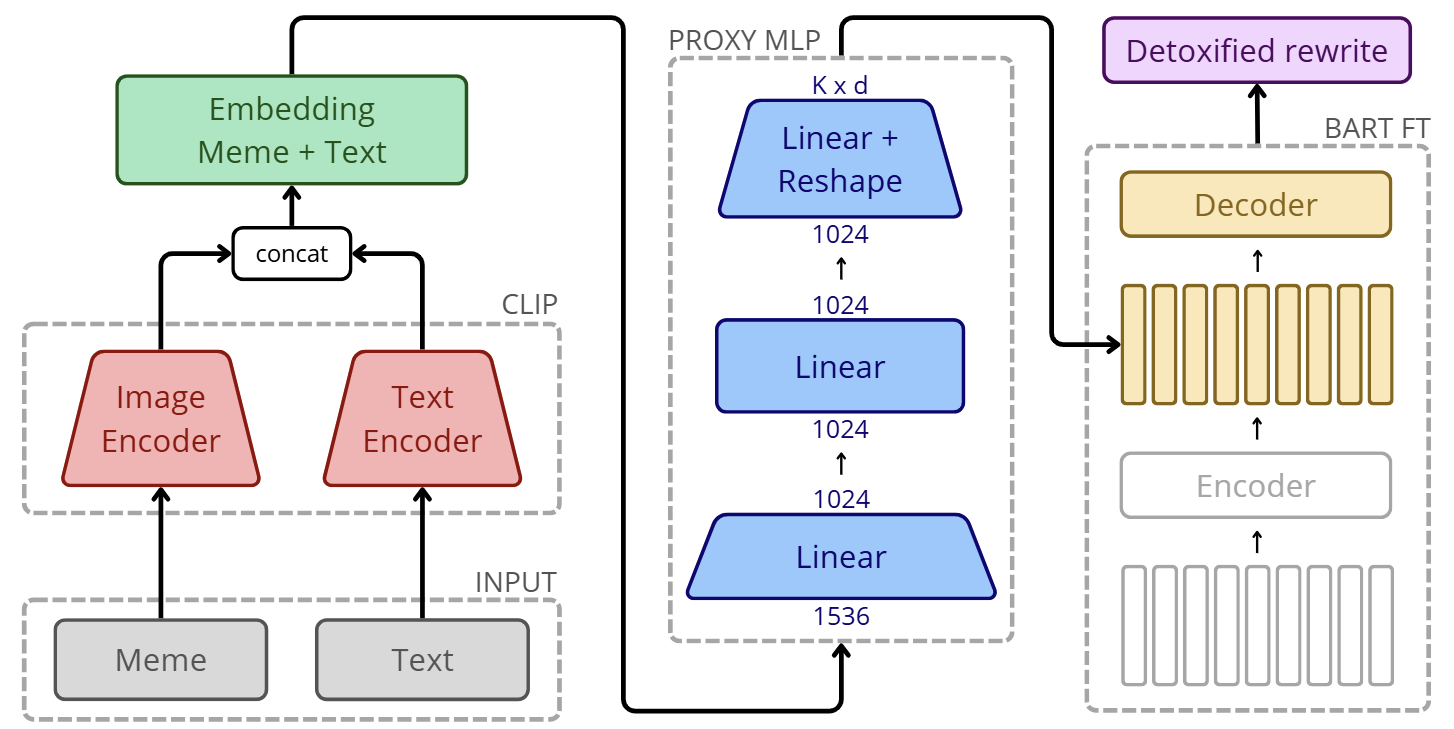
\includegraphics[width=1\columnwidth]{../inference.png}
\caption{Efficient inference path: the proxy maps CLIP meme/text embeddings to
BART soft encoder tokens for detoxified decoding.}
\label{fig:inference}
\vskip -0.12in
\end{figure}

\section{Data Licensing and Ethics}
\label{sec:ethics}

The project uses only public or research-access datasets already documented in
the repository materials. Those materials identify HarMeme and MAMI as CC~4.0
research datasets; the pipeline downloads HarMeme automatically, documents MAMI
as a manual-request dataset, and uses MMHS150K through the authors' research
download links rather than redistributing it. The paper reports aggregate
metrics and does not reproduce harmful images or captions.

Ethically, detoxification should be read as a harm-reduction tool, not as an
automatic moderation authority. Rewriting can remove slurs while still
preserving stereotypes, or it can over-neutralize legitimate counterspeech and
satire. Toxicity classifiers and hate datasets also encode annotation and
platform biases. For deployment, human review, uncertainty reporting, and clear
separation between educational research and real moderation decisions would be
required.

\section{Experiments and Results}
\label{sec:experiments}

All systems are evaluated on the same 280 held-out test examples with the same
scoring pipeline and exact generated outputs: no manual correction or post-hoc
sanitization is applied before scoring. Baselines are the fixed LLaVA teacher
pseudo-rewrites, a single reported DetoxLLM-7B run, and base BART. 
Metrics are Text \sta{} (mean non-toxic probability from a RoBERTa classifier), \sta{} delta (rewrite \sta{} minus original \sta{}), BERTScore F1, and normalized CLIPScore. Higher is better for all metrics. BART-FT results are averaged across five seeds with different random initializations of the LoRA parameters, while LLaVA and DetoxLLM are single runs because of computational cost. The proxy is trained on the same five BART-FT seeds and evaluated on the same test set, so its mean and standard deviation reflect the underlying BART-FT variance rather than separate random seeds for the proxy itself.
\begin{table}[t]
\vskip -0.06in
\centering
\scriptsize
\setlength{\tabcolsep}{1.6pt}
\begin{tabular}{@{}lcccc@{}}
\toprule
System & Text \sta{} & \sta{} $\Delta$ & SIM & CLIP \\
\midrule
LLaVA teacher$^\ast$ & \best{0.990} & \best{0.234} & 0.472 & 0.636 \\
DetoxLLM-7B$^\dagger$ & 0.940 & 0.184 & 0.443 & 0.634 \\
\bartft{} full & 0.963$\pm$0.006 & 0.207$\pm$0.006 & 0.330$\pm$0.013 & 0.628$\pm$0.001 \\
\bartft{} target & 0.960$\pm$0.005 & 0.204$\pm$0.005 & 0.335$\pm$0.013 & 0.629$\pm$0.002 \\
\bartft{} visual & 0.960$\pm$0.004 & 0.204$\pm$0.004 & 0.284$\pm$0.080 & 0.624$\pm$0.007 \\
\bartft{} none & 0.957$\pm$0.013 & 0.201$\pm$0.013 & 0.325$\pm$0.030 & 0.628$\pm$0.002 \\
Proxy+BART & 0.884$\pm$0.015 & 0.128$\pm$0.015 & \best{0.581$\pm$0.020} & \best{0.638$\pm$0.002} \\
\bottomrule
\end{tabular}
\caption{Test results on 280 memes. Rows with $\pm$ are seed 1--5
mean$\pm$sample std; $^\ast$LLaVA is a fixed teacher target and
$^\dagger$DetoxLLM is a single reported run.}
\label{tab:results}
\vskip 0.12in
\end{table}

Table~\ref{tab:results} shows that, across five BART seeds, all \bartft{}
variants obtain higher mean Text \sta{} and \sta{} delta than the single
reported DetoxLLM baseline. The \texttt{full} condition has the best average \bartft{}
detoxification, while \texttt{target\_only} is close and has the best BART-only
SIM. The ablation study suggests that the conditioning is not crucial for detoxification.

The external comparison and base-model ablation support the need for
meme-specific fine-tuning. Base BART reaches high non-toxicity in the full
condition (0.973 text \sta) but has negative SIM (-0.061), indicating generic
safe text rather than faithful rewriting. DetoxLLM keeps higher SIM than the
BART-only students (0.443 vs. roughly 0.33), but
copying can inflate BERTScore when toxic input is retained. Similarity must
therefore be interpreted together with Text \sta{} and \sta{} delta, not as a
stand-alone quality score.

The proxy exposes the deployment trade-off. It obtains the best mean SIM
(0.581) and CLIPScore (0.638), suggesting stronger source retention and image
alignment, but its Text \sta{} drops to 0.884. This can partly reflect
retention of harmful content, so the proxy is not the strongest detoxifier. Its
advantage is architectural: it uses CLIP plus a small MLP and BART decoder, not
LLaVA. In our A100 benchmark, BART-FT requires 122 ms per rewrite, compared
with 9.38 s for the LLaVA teacher and 1.99 s for DetoxLLM. The proxy
evaluation took 3.4 minutes for 280 examples, about 0.73 s/image, roughly
13$\times$ faster than LLaVA and 2.7$\times$ faster than DetoxLLM.

\vspace{0.28em}
\noindent\textbf{Limitations.} The project depends on LLaVA pseudo-labels rather than
human detoxification references, and the heterogeneous source datasets remain
noisy even after filtering. We do not include human evaluation; automatic
toxicity, BERTScore, and CLIPScore may miss pragmatic harm, counterspeech,
satire, or cases where lexical similarity preserves the harmful implication.
The BART student without the proxy receives visual context only as teacher text
fields, not pixels.
Finally, the proxy is not yet a drop-in replacement: it preserves similarity and
alignment, but its lower Text \sta{} requires stronger toxicity control.

\section{Conclusion}
\label{sec:conclusion}

We reframed harmful meme moderation as constructive text rewriting. A
LLaVA-NeXT teacher supplies multimodal explanations and pseudo-rewrites, while a
LoRA-adapted BART-large student is the strongest detoxification student in our
evaluation relative to the single reported DetoxLLM-7B baseline. The CLIP Proxy
+ BART path is the novel efficient deployment route: it removes large VLM/LLM
inference and improves fidelity metrics, but future work must improve proxy
toxicity control while preserving efficiency and image alignment.

\renewcommand{\bibfont}{\footnotesize}
\setlength{\bibsep}{1pt plus 0.3ex}
\bibliographystyle{ieeetr}
\bibliography{main}

\end{document}
